\documentclass[12pt]{article}

\usepackage[utf8]{inputenc}

\usepackage{graphicx} % Required for inserting images

%\usepackage[legalpaper, margin=0.9in]{geometry}
\usepackage[margin=0.9in]{geometry}
\usepackage{setspace}
\setlength{\parskip}{0pt}

%\usepackage{bookman}

\usepackage{amsmath,amssymb}
\usepackage{amssymb}
\usepackage{amsmath}

\usepackage{longtable}


\usepackage{lscape}
\usepackage{booktabs,caption}
\usepackage{hyperref}
\usepackage[authordate,backend=biber]{biblatex-chicago}
\usepackage[flushleft]{threeparttable}
\usepackage[T1]{fontenc}
\usepackage{palatino}
\usepackage{soul}

\setlength{\parskip}{0pt}

\usepackage{kotex}

\usepackage{biblatex}
\usepackage[authordate,backend=biber]{biblatex-chicago}
\addbibresource{bib.bib}



\usepackage{hyperref}
\hypersetup{
    colorlinks=true,
    linkcolor=blue,
    filecolor=magenta,      
    urlcolor=cyan,
    allcolors=blue
    }





\begin{document}
\setcounter{page}{0}



%\title{\textsc{Do Surprise Signals of Firms Affect Firms' Performance?}} \\ \\ \large{\fontfamily{qpl}\selectfont{: The Impact of Bonus from Tax Reform on Airline Product Quality}}}

\title{\Large{\textsc{{\textbf{A Study on the Fuel Price Competition
}}\\
\large{in the Korean LNG Electricity Generation Market}}}}

%\iffalse
\author{Junyeol Ryu\footnote{Department of Economics, University of Oklahoma, Email: junyeol.ryu-1@ou.edu}, }
%\fi

\setlength{\parskip}{1.5\baselineskip}

\date{May 2024}
\maketitle
\doublespacing
\setlength{\parskip}{0pt}

\singlespacing
\textbf{Abstract:} 
This study empirically analyzes the effect of introducing competition in the LNG market. Using confidential electricity generator data, we try to examine whether private electricity generators directly importing LNG are advantageous in terms of cost compared to generators importing LNG from public government corporations. The result indicates that a private firm's strategic behavior leads to cost-effective fuel prices but causes unexpected consequences in the market. In addition, this study investigates the effect of government intervention and infrastructure and provides policy implications for problems and consequences of the introduction of competition. 

\\

\noindent \textbf{Keywords:} LNG, 
\\





\newpage
\doublespacing

\section{Introduction}

In the global LNG market, the Seller's market, where suppliers have an advantage according to supply and demand conditions, and the Buyer's market, where consumers have an advantage, have been repeated \footnote{Buyer's market and Seller's market are terms representing LNG supply and demand conditions and prices, and are mainly used by LNG market research.}. The buyer's market has a low LNG spot market price due to a high LNG supply (oversupply) or lack of demand, and the Seller's market has a high LNG market price due to a lack of LNG supply or high demand. 

Korea's LNG generators compete for fuel price(cost) and efficiency in the cost-based pool (CBP) electricity generation market and are mainly responsible for the peak load. Until now, most electricity generators using LNG in Korea have been supplied with LNG from the Korea Gas Corporation, which is commonly called "KOGAS" \footnote{In South Korea, the Korea Gas Corporation, a public corporation, has been exclusively in charge of overseas introduction and domestic wholesale supply of LNG. Since 2005, direct-import generators for self-consumption have been allowed for the purpose of deregulation of the gas industry and the burden of public investment, and direct imports have increased in the total introduction of Korean LNG since 2015, accounting for 22.9\% of the total introduction in 2020.}. Meanwhile, since the start of the Buyer's market, which has had a low global LNG market price since 2015, the number of generators that directly purchase and procure LNG from overseas without receiving LNG for electricity generation from KOGAS has been increasing. This is in accordance with the purpose of securing a cost advantage in electricity generation using LNG from 2015.

KOGAS, which supplies about 82\% of LNG introduced to Korea, values stable procurement of supplies. Therefore, it is characterized by a high proportion of long-term contracts based on oil price linkage that can stably procure the quantity. On the other hand, it is known that private direct-import electricity generation companies are very sensitive to the introduction of LNG spot prices and have a low proportion of long-term contracts compared to KOGAS because they pursue profits. Consequently, private direct-import electricity generation companies have a high proportion of the LNG spot market. In particular, it has been known that in the buyer's market, private direct-import electricity generators showed a cost advantage over KOGAS generators because the spot market price is low. However, as the global LNG market was converted to the seller's market due to the energy crisis that occurred before and after the outbreak of the Russian-Ukraine War, the LNG spot market price rose to the highest level, and the high price continued. During this period, KOGAS electricity generators with a small proportion of the spot volume will have a cost advantage over direct-import generators.

The purpose of this study is to analyze empirically whether private electricity generators directly importing LNG are advantageous in terms of cost during the Buyer's market period in the Korean electricity market and whether KOGAS generators are advantageous in terms of cost in the Seller's market. Chapter 2 will explain the current status of Korea's LNG introduction competition and electricity generation market.  Chapter 3 examines literature studies related to the natural gas pricing mechanism and gas introduction competition. In the analysis part of Chapter 3, we will distinguish between Buyer's market and Seller's market with Asian LNG price (JKM, Japan Korea Market) from January 2015 to May 2023, using Bai Parron's test to determine whether there is a structural change in market price. In chapter 4, We discuss the data and empirical approach, and chapter 5 provides empirical results. The last chapter will discuss this study's main results and implications.





\newpage
\section{Institutional Background}

Korea began introducing LNG in 1987 as part of its efforts to diversify energy sources after the first and second oil shocks, and as of 2022, it is the world's third-largest importer of LNG after Japan and China. Korea consumed 45.4 million tons of LNG in 2022, with 51\% of its total consumption used for electricity generation and 49\% for city gas. In Korea, the Korea Gas Corporation(KOGAS), a public corporation, has been in charge of overseas introduction and domestic wholesale supply of LNG. It is responsible for 81.9\% of domestic LNG imports, 86\% of terminal capacity, and 100\% of the high-pressure pipe network. Since 2005, Korea has allowed direct imports for self-consumption for the purpose of deregulation of the gas industry and the transition of the burden of public investment, and the share of direct imports in total LNG imports has increased from 4.3\% in 2005 to 22.9\% in 2020.

For the past 20 years, the international LNG market has repeatedly experienced a phenomenon in which LNG market prices periodically increase (seller market) or decrease (buyer market) depending on supply capacity and demand. From 2011 to 2014, a seller market was formed in which LNG prices soared due to an increase in demand for Japanese LNG due to the Fukushima nuclear crisis, expectations for global economic recovery, and growth prospects in emerging LNG markets, including China. Since 2015, long-term global economic growth has slowed, leading to a decrease in LNG consumption in major countries, and the buyer market continued until mid-2021. From the second half of 2021, the seller market resumed in the aftermath of the Russia-Ukraine War.

As shown in Figure1 \footnote{Data Source: S\&P 2024, Global Commodity Insights, Japan Ministry of Finance, China Customs}, from 2015 to mid-2021, the LNG market formed a buyer's market, and the spot price of LNG was formed lower than the oil price. Korea's direct import of LNG has increased rapidly after the buyer's market. This is in accordance with the purpose of securing cost competitiveness in the electricity generation market by directly introducing inexpensive LNG in the global market.




KOGAS is the only LNG wholesaler in Korea, and KOGAS generator has a duty to secure and supply LNG. Therefore, for a stable supply of gas, it has a high proportion of long-term contracts related to oil prices and a low proportion of spot goods. On the other hand, private direct-import electricity generators do not have a separate stockpile obligation because they introduce LNG for the purpose of pursuing profits, and generally have a lower proportion of long-term contracts and a higher proportion of spot goods than KOGAS generators.

The KOGAS signed long-term contracts with overseas LNG suppliers in consideration of total consumption without classifying LNG introduced to Korea by use(residential, industrial, electricity generation), and introduced additional  LNG in spot market for the excess of winter heating demand. By introducing both electricity generation and city gas simultaneously, LNG demand for electricity generation played a role in mitigating the high and low characteristics of city gas demand, enabling long-term contracts and efficient storage tank operation, and contributing to the expansion of city gas demand. As a result, the LNG introduction price of the KOGAS has calculated the fuel price by dividing the sum of the payment amount for the long-term and short-contract volume by the total introduction volume, which is called the average price system. On the other hand, since direct importers individually introduced LNG from overseas, the fuel price of direct-import generators is calculated differently depending on the conditions of the introduction contract.


Competition has been introduced and operated in the Korean wholesale electricity market by separating the electricity generation sector of Korea Electric Power Corporation(KEPCO), a former vertical monopoly, establishing six subsidiaries and allowing private electricity generation companies (IPP) to enter new markets. In the Korean electricity market, electricity generation companies are competing in a cost-based pool (CBP) system, in which electricity generation capacity is bid based on the cost determined for each generator by the Cost Evaluation Committee one month in advance, not the price \footnote{fuel price, main variable in this paper, is the cost to determine operation.} 


In the Korean electricity market, various electricity generation sources, such as renewable, nuclear, coal, LNG, and oil, are participating in the electricity generation sector. However, due to the distinct difference in fuel prices between nuclear, coal, LNG, and oil electricity generation sources, competition between electricity generation sources is not possible. Electricity generation is taking place in the form of nuclear, coal, and renewable energy generators taking charge of the base load, and LNG generators taking charge of the peak load. LNG generators determine 82.5\% of the annual hourly electricity market price.

Competition among LNG generators is taking place through fuel price(cost) and generator efficiency. When most LNG generators receive LNG from KOGAS, the Korean LNG electricity generator using LNG competes through its heat efficiency. Since the fuel price has remained the same in the meantime, the electricity supply priority and electricity generation were determined by the generator's efficiency. However, with the emergence of private electricity generators that directly import LNG after 2015, competition patterns changed to fuel price competition between direct-import generators and KOGAS generators. Even if the efficiency of the generator is, they will be able to compete in terms of electricity generation costs if LNG is introduced at a low cost.


\newpage
\section{Literature Review}


\subsection{LNG Pricing Mechanism}
There has been continuous discussion on which natural gas pricing mechanism is more efficient. Natural gas pricing mechanisms can be largely divided into gas-on-gas prices, linked oil prices, and government-regulated prices (\cite{hupka2023review}).

Many studies show that gas market prices are more suitable as a pricing mechanism than price-linked oil. Supporters of gas market prices argue that gas market prices better reflect the market's supply and demand conditions and that price fluctuations are less extreme than linked oil prices. In particular, in LNG transactions, gas market prices such as JKM are more efficient with long-term contract prices than linked oil prices (\cite{zhang2023revisiting}, \cite{alim2018asian}). In addition, some studies have suggested that the role of oil prices as a major driver of natural gas prices in the two markets is weakened through the gradual transition to hub gas prices in Europe and the increase in spot trading in the Asian LNG market (\cite{zhang2018exploring}). \cite{stern2020comparative} shows that LNG deliveries traded short-term to Asia are increasingly priced at JKM and are not oil price indexing

On the other hand, studies support the efficiency of oil price-linked prices as a gas pricing mechanism. In a review of early studies on LNG, \cite{hupka2023review} suggests that there is strong evidence of the co-movement between LNG prices and crude oil prices before a series of structural breaks. \cite{komlev2016oil} argues that, first, because most long-term gas contracts are linked to oil prices, hub-based prices can only represent the remainder of the volume traded at oil-based prices; second, since oil-based prices act as price anchors for hub-based prices, hub-based prices are more likely to fail in the market; and finally, the amount of gas traded with crude oil price links is larger than hub-based prices, making it less likely to be manipulated.\cite{zhang2018exploring} states that oil-based prices are not the only factor in determining LNG prices even in Asia, where large amounts of LNG transactions are made at oil-based prices, but Asia expects oil-based pricing to remain dominant and difficult to change in the short term.




\subsection{LNG Introduction Competition in Electricity Market}

Literature studies on the introduction and competition of natural gas by companies are very scarce \footnote{In most cases, gas supply prices and methods of gas supply are not disclosed to the outside as corporate secrets, making it difficult to conduct related empirical research}.

\cite{fernandez2020analysis} evaluates whether electricity generation companies have an incentive to procure natural gas for electricity generation at a socially optimal level through the equilibrium model based on the Chilean electricity market. Research has shown that strategic companies can have an incentive to exercise market power by contracting a smaller amount than the socially required optimal amount of imports.


A number of prior studies related to the efficiency of companies' LNG introduction methods in the electricity market can be found in Korean academia \footnote{In the Korean electricity market, there is no contract transaction between electricity generators and sellers, all electricity transactions are made at Cost Based Pool, and market transaction information is disclosed because all LNG generators compete for fuel cost and electricity generation efficiency in this pool.}.

Son et al. 2009 show that private direct-import electricity generators generate and bid for electricity by profit motivation, and contribute significantly by lowering market prices to the electricity market based on fuel costs introduced at a low price.

Kim et al. 2009 analyzed the determinants of natural gas introduction by private direct importers in Korea, and the result indicates that contract price is the most important factor to consider. Private direct importers are considering strategies to maintain the competitiveness of direct imports through price changes if necessary, maximize the advantage in favorable environments through volume adjustment, and minimize risk in unfavorable environments.

Lee et al. 2018 argue that there is an imbalance between opportunities and risks between the KOGAS generators and the direct-import generators in terms of gas introduction competition in the Korean electricity market. While direct-import generators can strategically choose whether to introduce spot supplies in consideration of the impact of the introduction of spot supplies on the cost of generators in the electricity market, the KOGAS generators, which are responsible for the stable supply of all consumers in the regulated market, emphasizes the stable procurement of the quantity demanded by consumers. As a result of the combination of the characteristics of the Korean gas market and the electricity market, direct importers can get an opportunity to reduce raw material costs and expand profits in the electricity market by actively introducing low-cost spot goods while avoiding the introduction of expensive spot goods. On the other hand, KOGAS, which is obligated to supply and demand the entire country, introduces expensive spot goods compared to direct import operators, resulting in an increase in raw material costs for electricity generation.

Doh et al. 2021 argue that direct imports, which have a high proportion of spot introduction in Korea's LNG introduction market, show a cost advantage over KOGAS generators in the Buyer's market.




\newpage
\section{Data and Empirical Strategy}

\subsection{Data Description}
The purpose of this study is to empirically analyze whether generators directly importing LNG are advantageous in terms of cost during the Buyer's market period within the Korean electricity market and whether KOGAS generators(importing jointly) are advantageous in terms of cost in the Seller's market. 8,420 panel data per month for 91 LNG generators were constructed from January 2015 to May 2023. The data is from the Korea Electric Power Corporation(KEPCO) and consists of the generator name, year, month, monthly fuel price for generators in generating electricity, generator type, fuel introduction method (KOGAS; average price, Private; direct import, Combination; both), JKM price, JCC price, HH price, terminal ownership, and generator capacity. There are 800 data for the direct-import method, 7,428 data for the average price system for KOGAS, and 192 data for combination. The table1 provides basic statistics on 8420 data used in this analysis. The average fuel price for the entire sample period was 64 won(₩, which is a Korean currency unit), JKM was 12 dollars, and JCC was 10 dollars.



The fuel price can be defined as 'the fuel price for generating the unit heat of each generator' and is composed of 1) raw material cost and 2) the supply cost. The raw material cost is the price of LNG introduction. The supply cost is calculated based on the LNG terminal rate and the piping cost. Of the total fuel price, the proportion of raw material accounts for 90\%, and the proportion of supply cost accounts for about 10\%, indicating that the influence of raw material is absolute.

Figures 2 and 3 show 1) JKM and fuel price distribution according to three types of LNG introduction methods(Private Direct Import / KOGAS average price system / Combination) and 2) JCC and fuel price distribution. Consistent with our intuition, the fuel price of the generator with the KOGAS average price system was relatively less dispersed than that of the generator with a Private direct-import.
This is due to the characteristics that companies and generators that import LNG from the average price system of KOGAS import LNG volume at a relatively stable price through long-term contracts. However, Private generators that directly import LNG concentrate on relatively short-term volumes, and each company and generator's purchase timing and market conditions differ at the time of purchase, making the price dispersion relatively large.



In addition, when comparing the distribution of JKM \& fuel price and the distribution of JCC and fuel price, the relationship between the energy price and fuel price (positive, +) was more clearly shown with JCC. Compared to JKM, which relatively affects short-term LNG contracts, JCC has a linear and more predictable effect on fuel price as an JCC greatly affects LNG long-term contracts.



\subsection{Dividing Buyer's-Seller's Market using Bai-Perron Method}

In this study, the Bai-Perron (1998, 2003) test was used to analyze whether there was a structural change in the LNG spot market price using monthly data of the JKM(Asian LNG spot price, Japan-Korea Marker) from January 2015 to May 2023. The figure4 visualizes the price trend of JKM. Starting in mid-2021, JKM prices have risen sharply. This coincides with the time when international natural gas prices soared due to the suspension of supply of the Yamal-Europe gas pipeline, one of Russia's export gas pipelines to Europe, in December 2021 and the outbreak of the Russia-Ukraine war in February 2022.







The table2 shows the optimal number of structural changes in the JKM price trend estimated through the Bai-Perron test\footnote{As a result, from January 2015 to May 2023, SSR value was 3238.99, and it was estimated that structural changes occurred between May 2021 and July 2021 with a 95\% confidence interval.}. The Bai-Perron technique(\cite{bai1998estimating}, \cite{bai2003computation}, \cite{bai2003critical}) identifies the time point when structural breaks appear in time series data. In this paper, the number and timing of structural changes were estimated under the assumption that not only the time point of structural change within the JKM price but also the number of structural changes is not determined. Thus, we estimate the optimal time point and a number of structural changes through Bai-Perron, and we subdivided the market based on that point (Seller's market and Buyer's market) to analyze the effect of LNG introduction import methods on fuel price in a multi-layered. 

As a result of the Bai-Perron test, the most suitable number of structural breaks in the monthly JKM price trend from January 2015 to May 2023 was found to be one (one-time point), and the time point was estimated to be June 2021\footnote{The statistical significance of dummy variables can be confirmed by adding dummy variables to the model to divide the time of structural change if the time point is explicitly known or the time point is determined by the researcher. However, this analysis assumes that the time point and the number of structural changes are not determined. Thus, we estimate using monthly JKM data.}. The Bai-Parron result that the structural change occurred in June 2021 can be seen as consistent with the JKM price trend that has been soaring since mid-2021 in Figure 4. Accordingly, the time of structural change in JKM prices was set at June 2021, and from January 2015 to May 2021, the buyer's market was set where LNG prices were low, and buyers had an advantage, and from June 2021 to May 2023, the seller's market where LNG prices were high.



\subsection{Empirical Approach}

In this study, the regression model is set as the model to analyze which method is more cost-effective for the fuel price between the direct introduction by private generator, the average price system by KOGAS generator, or the combination method.



\begin{align*}
Y_{i}  = \beta_0 + \beta_1 Direct Import_{i} + \beta_2 Combination_{i} + \alpha X_{i}+ \delta_{type} +  \theta_{time} + \epsilon_{i}
\end{align*}


The dependent variable (fuel price), {$Y$}, is the fuel price of each generator, the "DirectImport" variable represents the case where generators directly import LNG, and the "Combination" variable represents the case where generators import LNG with KOGAS method and Direct Import method. The generator with the "KOGAS" average price system, which is not included in the model, is a comparison group, and the estimated coefficients of {$\beta1$}  and {$\beta2$} show how cost-effective the direct introduction generator and the combined generator are compared to the fuel price of the KOGAS generator.

The {$X$} is control variables that represent the factors affecting the dependent variable, the fuel price. Since the purpose of this analysis is to estimate the effect of direct introduction on fuel price, other factors on fuel price should be sufficiently controlled to secure the reliability of the results. Various variables are controlled by adding JKM price, JCC price, generator capacity, operation start Day, and HH price to the model that affect the fuel price.


In addition, the model includes a time-fixed effect and a generator-type fixed effect. When the unobserved individual-specific characteristics affect the dependent variable, the endogenous problem can be alleviated by controlling the unobserved individual-specific characteristics with a fixed effect. The fuel price, the dependent variable of this analysis, is largely determined by the raw material cost and the supply cost, and the supply cost is greatly affected by the season. Therefore, the characteristics of the season influence supply cost, making a difference in fuel cost. In addition, generator types consist of CHP(combined heat and power) and CCP(Combined cycle power generation), and the unique characteristics of each generator type can structurally affect the fuel price. Accordingly, the year-season fixed effect and generator type fixed effect were included in the model to control the effect of time and generator type on fuel price, respectively. Figure 5 shows different fuel price according to the season\footnote{The fuel price by season was found to be 65.18 ₩ in spring, 54.87 ₩ in summer, 62.58 ₩ in autumn, and 70.25 ₩ in winter.}


On the other hand, in this model, the each generator fixed effect was not applied. Since most generators introduce LNG only in one way by either the direct import method or the KOGAS average price system, applying the fixed effect for each generator will result in enormous data loss. Instead of setting a fixed effect for each generator, the analysis tries to control factors that affect fuel price. As discussed, the fuel price is 90\% determined by the raw material cost, and the remaining 10\% is determined by the supply cost. The impact of raw material cost on fuel price was controlled by including the JCC and JKKM price index, and since the supply cost is caused by seasonal fluctuations, the effect of supply cost can be sufficiently controlled by adding a year-season fixed effect to the model.












\newpage
\section{Result}

\subsection{Basic Finding}



The table3 shows the results of the basic regression analysis. Column (1) included raw material costs such as JKM and JCC. As mentioned earlier, since the fuel price is greatly affected by the price of raw materials, control of raw material cost is essential for estimation. Column (2) further included generator capacity interval\footnote{The generator capacity was grouped based on 100 by size, and a total of 9 generator capacity categories were created and a fixed effect was applied.}. Since variation in generator capacity may directly or indirectly affect the fuel price, the capacity interval variable was controlled. In column (3), the generator capacity level variable was included in the model. In column (4), instead of the year-season fixed effect, a year-month fixed effect was applied. 
As a result of all four analyses, the fuel price of the generator that directly imports LNG is found to be significantly more cost-effective than that of the KOGAS(average price system) generator, and the fuel price of the generator that uses two methods(combination) is also significantly cost-effective than that of KOGAS, but the effect is relatively small.
JCC affects the fuel price more than JKM, and generator capacity was found to have no significant effect on it. The analysis to be discussed uses the results derived in column (3) as the basic result.










\subsection{Comparison between Buyer's Market and Seller's Market}

The table 4 analyzes the LNG market by dividing it into a buyer's market with low JKM gas prices and a seller's market with high gas prices as of June 2021, based on the time of structural change derived according to Bai-Perron. As a result, the fuel price of a direct import generator is estimated to be more cost-effective than that of a KOGAS generator in both the buyer's market and the seller's market.
Interestingly, in Seller's Market, where gas market prices are high, direct import generators have a lower fuel price than KOGAS generators, and the fuel price reduction effect was even greater compared to Buyer's market. This is inconsistent with our intuition and requires an in-depth discussion.



Looking at the Long and Short-term Contracts table5 \footnote{LNG Trade Tables from S\&P Global(2024.1.26).} in the KOGAS generator, the proportion of long-term contracts decreased, and the proportion of short-term increased in 22 years compared to 21 years. Conversely, direct-import generators have increased the proportion of long-term contracts and decreased the proportion of short-term.

This means that direct-import generators can adjust their portfolio by changing the proportion of long-term and short-term contracts in the Seller's market since the spot gas price is high in that period, but the KOGAS generator, which should supply the entire LNG, cannot adjust its volume portfolio according to the market situation, and if additional supplies are needed to meet the national gas supply and demand, the KOGAS has to increase spot purchases even though it is Seller's market. As a result, the fuel price of the KOGAS generator continues to be higher than that of direct-import generators not only in the Buyer's market but also in the seller's market.
Therefore, private generators(direct-import generators) were able to achieve cost efficiency through strategic behavior under the market structure, and the KOGAS generators are more difficult to achieve cost efficiency due to restrictions on the securing of LNG supplies.





\subsection{Price Cap Regulation Impact}

Due to the surge in energy prices, the Korean electricity market applied a price ceiling system in December 2022, January, February, and April 2023. Generators participating in the Korean electricity market, including LNG generators, will be compensated only up to the notified upper limit. According to a price cap regulation, direct-import generators have the incentive to give up profits by increasing the fuel price during the price cap regulation period \footnote{The Korean electricity market determines and commands the order of operation of the generator based on the fuel price. In other words, if the fuel price is cheap, the probability of operation of the generator is high, otherwise, the probability of operation of the generator is low.}. In other words, generators have an incentive to out the operation by making fuel prices high because, in the price cap regulation period, their profits are expected to be low.

In Table6 \footnote{Since the application of the price cap is after December 2022, the period was limited to the seller market.}, the direct-import generator during the regulation period still showed a more cost-effective fuel price than that of the KOGAS generator, but the fuel price efficiency was reduced compared to fuel price in the nonregulation period. This result can be seen as a consequence of the government's sudden intervention in the market, which reduced the cost-efficiency effect of direct-import generators. The government's rapid intervention can induce each market player(private firms) to take strategic actions to maximize profits, resulting in negative consequences that were not originally intended for market efficiency and stability.






\subsection{Terminal Ownership Effect}

Having a terminal means that fuel supply volume and transportation adjustments can be made more efficiently and flexibly according to market conditions. The terminal retention effects can be summarized into three categories.
First, it is less sensitive to fuel price volatility and can reduce fuel purchase costs. Second, it can lower operating costs by reducing logistics costs related to fuel transportation. Third, it is easy to sign long-term contracts with LNG suppliers, which can help secure fuel at a stable price.
Consequently, this subsection focuses on the terminal ownership effect, as it can significantly affect the fuel price of the generator.

The table7 analyzes the effect of terminal ownership. As a result, the fuel cost of direct-import generators with a terminal is found to be more cost-effective in both markets, and the effect is especially remarkable in the seller's market. In other words, the cost-effectiveness of fuel price by terminal ownership was more pronounced in the seller market, which suggests that in Buyer's market, where gas market prices are low, it is easy to supply inexpensive gas without a terminal, but in seller's market, where the gas prices are high, direct-import generators who own terminals can take advantage of terminal ownership to procure gas more efficiently.








\subsection{Robustness Checks}


The table8 shows the results of the model including the start of operation and the HH(Henry Hub) price instead of the JCC price. The start of operation year can be considered as an index that quantifies the degree of aging of the generator numerically so that individual characteristics of the generator can be controlled. In addition, since the HH price is an index that has a great influence on the long-term price of natural gas, it can control the characteristics of raw material cost that are different from those of JCC. 

As a result, the fuel price of the direct-import generator was found to be significantly more cost-effective than that of the KOGAS generator, which is consistent with the basic model. However, the start of operation did not have a significant effect on the fuel price.































\newpage
\section{Discussion and Conclusion}
In this study, we expected that private generators directly importing LNG with a low proportion of long-term contracts and a high proportion of spot goods would be advantageous in the buyer's advantage market and that generators importing from KOGAS with a high proportion of long-term contracts and a low proportion of spot goods would have a cost advantage in the seller's advantage market. This is because the spot gas market price is high in the seller's market and low in the buyer's market. However, contrary to our expectations, private generators directly importing LNG showed a cost advantage over KOGAS generators in both the buyer's market and the seller's market. The cost competitiveness was even higher in the seller's market. This can be interpreted for some reasons.

First, direct-import generators for the purpose of profit-maximizing purchased fuel more effectively in the seller's market. If spot prices are purchased at a time when the spot prices are as low as possible as the direct-import generator can choose the optimal timing of purchase while observing the price trend, the fuel price of direct-import generators can be lowered even if the proportion of spot prices in the total introduced volume is high \footnote{High spot prices show high and low volatility within the period}. 
On the other hand, for the KOGAS generators since securing stable supply and meeting demand is more important than profit-seeking, there is a possibility that the KOGAS generators purchased LNG at a high price to secure the quantity at a fixed time contracted in advance rather than at a low price while observing the price trend.


Secondly, under Korea's electricity transaction market, electricity generators that import LNG from KOGAS have a limit in that they cannot exhibit a cost advantage due to the structure in which the private direct-import generators can adjust their volume under the seller's market. Notably, direct-import generators have an incentive to reduce expensive spot supplies under the seller's market. Direct-import generators can adjust their portfolio by changing the proportion of long-term and short-term contracts, but KOGAS generators should secure the entire LNG, accordingly, they cannot adjust their volume portfolio. Even if a private generator reduces the short-term amount, the KOGAS generator must make up for the reduced short-term amount. Thus, unlike KOGAS generators, private generators(direct-import generators) can achieve cost efficiency through strategic behavior under the market structure. 

This study also examines the effects of factors such as government policies and infrastructure affecting the cost competitiveness of direct-import generators. First, we check the effect of the price cap regulation in the electricity market on fuel prices. Due to high energy prices during the energy crisis caused by the Russia-Ukraine war, several countries around the world took various measures to protect consumers. The price cap system implemented in Korea has been shown to reduce the cost efficiency of fuel prices. Second, we explore how holding LNG terminals affects the cost competitiveness of direct-import generators. Owning a storage space means being able to supply fuel flexibly according to market conditions rather than renting it. The result indicates that direct-import generators with terminals are shown to be more cost-effective. In fact, some firms considering a new direct-import electricity generator in Korea are also considering building a terminal. This can be consistent with our results. However, in the future, the increase in terminal construction lead to an excess of LNG storage space across the country, or the assetization of LNG infrastructure in the carbon neutrality process can be another debate.



Direct LNG imports are expected to increase further in the Korean LNG electricity generation market. In order to compete with direct-import generators, the Korea Gas Corporation(KOGAS) has also launched and operated a new contract type in which the KOGAS acts as a direct import agent. This means that in the future, Korea's LNG electricity generation market will become a more competitive market, pursuing cost efficiency rather than stabilizing supply and demand. However, there are several challenges. It is necessary to 1) establish the rule to operate the final supply and demand management 2) distribute the burden of supply and demand management currently borne by the KOGAS on direct-import generators, and the operation system of the electricity market requires various hedging means, long-term electricity supply contracts, contract for Difference, and price bidding.






\newpage
\printbibliography





\newpage
\section{Appendix}

\begin{figure}[htbp] 
    \centering
            \caption{Global Gas and LNG Prices(\$/MMBtu)}
        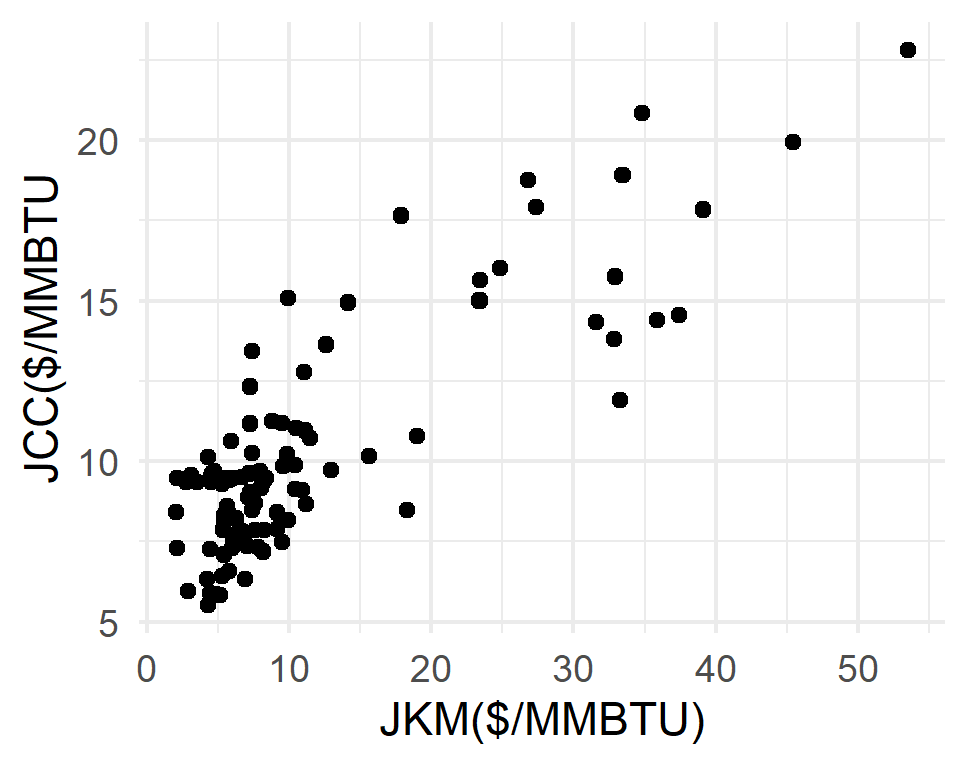
\includegraphics[width=0.8\linewidth]{Figure1.png}
        \label{fig:88mono}
\end{figure}




\begin{table}[htbp]\centering
\def\sym#1{\ifmmode^{#1}\else\(^{#1}\)\fi}
\caption{Summary Stats}
\begin{tabular}{l*{1}{ccccc}}
\toprule
\addlinespace
\textsc{Statistic}            &        \multicolumn{1}{c}{\textsc{Mean}}&         \multicolumn{1}{c}{\textsc{St. Dev.}}&        \multicolumn{1}{c}{\textsc{Min}}&         \multicolumn{1}{c}{\textsc{Max}}&           \multicolumn{1}{c}{\textsc{N}}\\
\hline \hline
\addlinespace
Fuel Price       &    64.03&    31.53&      16.89&       308.9&        8420\\
JKM         &    12.06&    10.79&       2.06&      53.51&        8420\\
JCC         &    10.48&    3.65&        5.52&        22.8&        8420\\
HH          &    3.29&    1.51&         1.7&        8.81&        8420\\
Capacity    &    421.19&    220.39&          21&         874&        8420\\
\bottomrule
\end{tabular}
\end{table}





\begin{figure}[htbp] 
    \centering
            \caption{Fuel Price and JKM(\$/MMBtu) by LNG Import Type}
        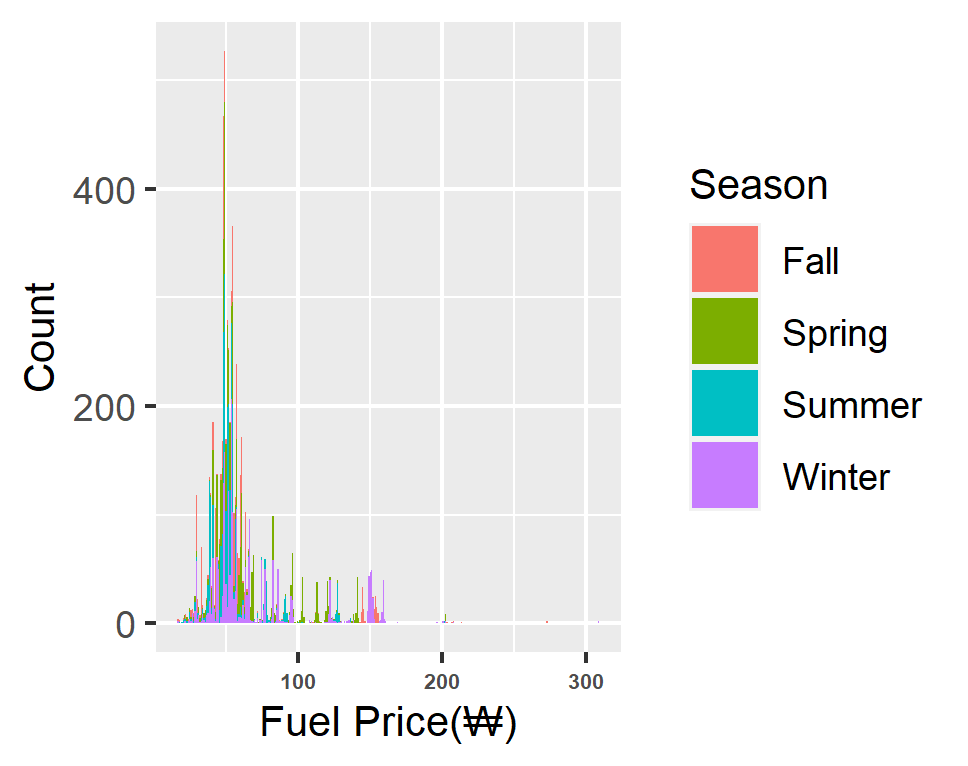
\includegraphics[width=0.5\linewidth]{Figure3.png}
        \label{fig:88mono}
\end{figure}




\begin{figure}[htbp] 
    \centering
            \caption{Fuel Price and JCC(\$/bbl) by LNG Import Type}
        \includegraphics[width=0.5\linewidth]{Figure4.png}
        \label{fig:88mono}
\end{figure}









\begin{figure}[htbp] 
    \centering
            \caption{JKM Price and Structural Break(\$/MMBtu}
        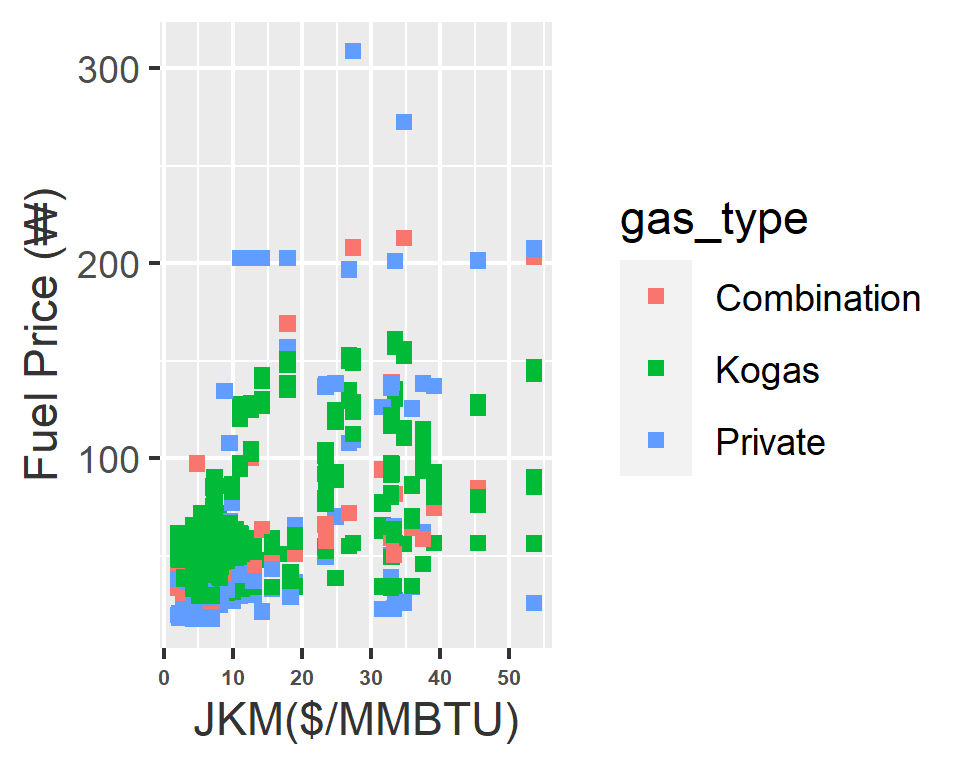
\includegraphics[width=0.6\linewidth]{Figure2.png}
        \label{fig:88mono}
\end{figure}




\begin{table}[htbp]\centering
\def\sym#1{\ifmmode^{#1}\else\(^{#1}\)\fi}
\caption{Bai-Perron Test}
\renewcommand{\arraystretch}{0.7}
\begin{tabular}{l*{4}{c}}
\toprule
 & \multicolumn{4}{c}{\textsc{Bai \& Paeron Critical Values}} \\ 
                                          \cline{2-5}  \\
                  &\multicolumn{1}{c}{\textsc{Test}}&\multicolumn{1}{c}{\textsc{1\% Critical}}&\multicolumn{1}{c}{\textsc{5\% Critical}}&\multicolumn{1}{c}{\textsc{10\% Critical}}\\             
                &\multicolumn{1}{c}{\textsc{Statistics}}&\multicolumn{1}{c}{\textsc{Value}}&\multicolumn{1}{c}{\textsc{Value}}&\multicolumn{1}{c}{\textsc{Value}}\\    


\hline \hline
\addlinespace
F(1|0)            &      108.70 &      12.29&      8.58 & 7.04\\

\addlinespace
F(2|1)                   &     9.44&      13.89&    10.13 &  8.51 \\

\addlinespace
F(3|2)                   &      1.57 &       14.80         &      11.14   & 9.41  \\

\addlinespace
F(4|3)                   &       5.97  &       15.28  &     11.83  &  10.04 \\

\addlinespace
F(5|4)               &      3.86         &      15.76&      12.25  &  10.58  \\

\midrule
Detected number of breaks   &   &    1 &    1 &    2  \\  
\midrule
\hline \hline
\end{tabular}
\end{table}







\begin{figure}[htbp] 
    \centering
            \caption{Fuel Price Histogram by Season}
        \includegraphics[width=0.5\linewidth]{Figure5.png}
        \label{fig:88mono}
\end{figure}










\begin{table}[htbp]\centering
\def\sym#1{\ifmmode^{#1}\else\(^{#1}\)\fi}
\caption{Main Result\label{tab1}}
\renewcommand{\arraystretch}{0.8}
\begin{tabular}{l*{4}{c}}
\toprule
 & \multicolumn{4}{c}{\textsc{Dependent variable}} \\ 
                     &\multicolumn{4}{c}{\textsc{:Fuel Price}}\\
                                          \cline{2-5}  \\
                    &\multicolumn{1}{c}{(1)}&\multicolumn{1}{c}{(2)}&\multicolumn{1}{c}{(3)}&\multicolumn{1}{c}{(4)}\\
\hline \hline
\addlinespace
\textit{Direct Import by private}              &     -10.851\sym{***}&     -10.720\sym{***}&     -10.818\sym{***}&     -10.834\sym{***}\\
                    &      (0.43)         &      (0.47)         &      (0.45)         &      (0.41)         \\
\addlinespace
\textit{Combination} &      -4.525\sym{***}&      -5.033\sym{***}&      -4.505\sym{***}&      -4.510\sym{***}\\
                    &      (0.85)         &      (0.88)         &      (0.85)         &      (0.77)         \\
\addlinespace
JKM                 &      -0.105\sym{**} &      -0.105\sym{**} &      -0.105\sym{**} &       \textit{omitted}         \\
                    &      (0.04)         &      (0.04)         &      (0.04)         &                 \\
\addlinespace
JCC                 &       6.036\sym{***}&       6.037\sym{***}&       6.036\sym{***}&       \textit{omitted}         \\
                    &      (0.21)         &      (0.21)         &      (0.21)         &                 \\
\addlinespace
Generator Capacity           &                     &                     &      -0.000         &      -0.000         \\
                    &                     &                     &      (0.00)         &      (0.00)         \\
\midrule
Year-Season FE         &    Yes &    Yes&    Yes&    No\\  
Generator Type FE        &    Yes &    Yes&    Yes&    Yes\\  
Generator Capacity Interval    &   No &    Yes&    No&    No\\  
Year-Month FE        &    No &    No&    No&    Yes\\  
Observations                   &    8420         &    8420         &    8420         &    8420         \\
$R^2$                   &       0.866         &       0.866         &       0.866         &       0.892         \\
\bottomrule
\multicolumn{5}{l}{\footnotesize Standard errors in parentheses.}\\
\multicolumn{5}{l}{\footnotesize \sym{*} \(p<0.1\), \sym{**} \(p<0.05\), \sym{***} \(p<0.01\)}\\
\end{tabular}
\end{table}






\begin{table}[htbp]\centering
\def\sym#1{\ifmmode^{#1}\else\(^{#1}\)\fi}
\caption{Buyer's and Seller's Market\label{tab1}}
\renewcommand{\arraystretch}{0.8}
\begin{tabular}{l*{3}{c}}
\toprule
 & \multicolumn{3}{c}{\textsc{Dependent variable}} \\ 
                     &\multicolumn{3}{c}{\textsc{:Fuel Price}}\\
                                          \cline{2-4}  \\
                  &\multicolumn{1}{c}{\textsc{Entire Sample Period}}&\multicolumn{1}{c}{\textsc{Buyer's Market}}&\multicolumn{1}{c}{\textsc{Seller's Market}}\\                                          
                    &\multicolumn{1}{c}{(1)}&\multicolumn{1}{c}{(2)}&\multicolumn{1}{c}{(3)}\\

\hline \hline
\addlinespace
\textit{Direct Import by private}               &     -10.818\sym{***}&     -10.079\sym{***}&     -12.695\sym{***}\\
                    &      (0.45)         &      (0.23)         &      (1.50)         \\
\addlinespace
\textit{Combination}  &      -4.505\sym{***}&      -2.654\sym{***}&      -8.418\sym{***}\\
                    &      (0.85)         &      (0.48)         &      (2.49)         \\
\addlinespace
JKM                 &      -0.105\sym{**} &       0.093\sym{*}  &      -0.355\sym{***}\\
                    &      (0.04)         &      (0.05)         &      (0.09)         \\
\addlinespace
JCC                 &       6.036\sym{***}&       3.740\sym{***}&       8.754\sym{***}\\
                    &      (0.21)         &      (0.13)         &      (0.56)         \\
\addlinespace
Generator Capacity          &      -0.000         &      -0.001\sym{**} &       0.002         \\
                    &      (0.00)         &      (0.00)         &      (0.00)         \\
\midrule
Year-Season FE        &    Yes &    Yes&    Yes\\  
Generator Type FE       &    Yes &    Yes&    Yes\\  
Observations                  &    8420         &    6244         &    2176         \\
$R^2$                  &       0.866         &       0.755         &       0.726         \\
\bottomrule
\multicolumn{4}{l}{\footnotesize Standard errors in parentheses.}\\
\multicolumn{4}{l}{\footnotesize \sym{*} \(p<0.1\), \sym{**} \(p<0.05\), \sym{***} \(p<0.01\)}\\
\end{tabular}
\end{table}


\begin{table}[h]
\centering
\caption{Long and Short-term Contracts}
\renewcommand{\arraystretch}{0.6}
\begin{tabular}{@{}ccccccccc@{}}
\toprule
YEAR & \multicolumn{3}{c}{KOGAS} & \multicolumn{3}{c}{Private Direct Import} & \multicolumn{2}{c}{Total} \\
\addlinespace
\hline \hline
\addlinespace
 & Long & Short & Total & Long & Short & Total & \\ 
\midrule
2015 & 26,021 (83.3) & 5,201 (16.7) & 31,222 & 1,195 (55.6) & 954 (44.4) & 2,148  & 33,371 \\
2016 & 26,813 (84.5) & 4,930 (15.5) & 31,742 & 1,273 (54.5) & 1,062 (45.5) & 2,335  & 34,078 \\
2017 & 29,232 (88.4) & 3,851 (11.6) & 33,083 & 2,567 (49.1) & 2,663 (50.9) & 5,230  & 38,313 \\
2018 & 31,469 (82.0) & 6,921 (18.0) & 38,389 & 2,576 (41.7) & 3,602 (58.3) & 6,178 & 44,568 \\
2019 & 28,363 (83.9) & 5,446 (16.1) & 31,809 & 2,645 (39.3) & 4,092 (60.7) & 6,737  & 40,547 \\
2020 & 27,272 (83.3) & 5,484 (16.7) & 32,755& 3,065 (37.9) & 5,015 (62.1) & 8,080  & 40,835 \\
2021 & 31,643 (82.4) & 6,772 (17.6) & 38,415 & 3,498 (44.1) & 4,441 (55.9) & 7,939  & 46,354 \\
2022 & 28,859 (71.9) & 11,280 (28.1) & 40,139 & 4,071 (58.4) & 2,898 (41.6) & 6,970  & 47,109 \\
2023 & 27,385 (74.1) & 9,590 (25.9) & 36,975 & 2,900 (35.6) & 5,247 (64.4) & 8,147  & 45,123 \\
\bottomrule
\end{tabular}
\end{table}








\begin{table}[htbp]\centering
\def\sym#1{\ifmmode^{#1}\else\(^{#1}\)\fi}
\caption{Price Cap Regulation in Seller's Market\label{tab1}}
\renewcommand{\arraystretch}{0.7}
\begin{tabular}{l*{1}{c}}
\toprule
 & \multicolumn{1}{c}{\textsc{Dependent variable}} \\ 
                     &\multicolumn{1}{c}{\textsc{:Fuel Price}}\\
\hline \hline
\addlinespace
\textit{Direct Import by private} &      -8.568\sym{**} \\
\textit{with Price Cap}                    &      (3.43)         \\
\addlinespace
\textit{Direct Import by private} &     -13.521\sym{***}\\
\textit{without Price Cap}   &      (1.62)         \\
\addlinespace
\textit{Combination}  &      -8.418\sym{***}\\
                    &      (2.49)         \\
\addlinespace
JKM                 &      -0.354\sym{***}\\
                    &      (0.09)         \\
\addlinespace
JCC                 &       8.741\sym{***}\\
                    &      (0.56)         \\
\addlinespace
Generator Capacity          &       0.002         \\
                    &      (0.00)         \\
\midrule
Year-Season FE          &    Yes \\
Generator Type FE        &    Yes \\
Observations                   &    2176         \\
$R^2$                 &       0.726         \\
\bottomrule
\multicolumn{2}{l}{\footnotesize Standard errors in parentheses.}\\
\multicolumn{2}{l}{\footnotesize \sym{*} \(p<0.1\), \sym{**} \(p<0.05\), \sym{***} \(p<0.01\)}\\
\end{tabular}
\end{table}







\begin{table}[htbp]\centering
\def\sym#1{\ifmmode^{#1}\else\(^{#1}\)\fi}
\caption{Terminal Ownership Effect\label{tab1}}
\renewcommand{\arraystretch}{0.6}
\begin{tabular}{l*{3}{c}}
\toprule
 & \multicolumn{3}{c}{\textsc{Dependent variable}} \\ 
                     &\multicolumn{3}{c}{\textsc{:Fuel Price}}\\
                                          \cline{2-4}  \\
                  &\multicolumn{1}{c}{\textsc{Entire Sample Period}}&\multicolumn{1}{c}{\textsc{Buyer's Market}}&\multicolumn{1}{c}{\textsc{Seller's Market}}\\                                          
                    &\multicolumn{1}{c}{(1)}&\multicolumn{1}{c}{(2)}&\multicolumn{1}{c}{(3)}\\

\hline \hline
\addlinespace
\textit{Direct Import by private}    &     -10.758\sym{***}&      -7.161\sym{***}&     -17.962\sym{***} \\
\textit{with Terminal Ownership}   &      (0.66)         &      (0.35)         &      (2.08)              \\
\addlinespace
\textit{Direct Import by private}&     -10.863\sym{***}&     -12.098\sym{***}&      -7.978\sym{***}   \\
\textit{without Terminal Ownership}  &      (0.58)         &      (0.30)         &      (1.98)            \\
\addlinespace
\textit{Combination} &      -4.502\sym{***}&      -2.438\sym{***}&      -8.514\sym{***}  \\
                    &      (0.86)         &      (0.47)         &      (2.48)          \\
\addlinespace
JKM                 &      -0.105\sym{**} &       0.093\sym{*}  &      -0.355\sym{***}  \\
                    &      (0.04)         &      (0.05)         &      (0.09)             \\
\addlinespace
JCC                 &       6.036\sym{***}&       3.738\sym{***}&       8.752\sym{***}  \\
                    &      (0.21)         &      (0.13)         &      (0.56)         \\
\addlinespace
Generator Capacity          &      -0.000         &      -0.001\sym{***}&       0.003             \\
                    &      (0.00)         &      (0.00)         &      (0.00)       \\
\midrule
Year-Season FE         &    Yes &    Yes&    Yes\\  
Generator Type FE        &    Yes &    Yes&    Yes\\  
Observations                    &    8420         &    6244         &    2176           \\
$R^2$                   &       0.866         &       0.760         &       0.728               \\
\bottomrule
\multicolumn{4}{l}{\footnotesize Standard errors in parentheses.}\\
\multicolumn{4}{l}{\footnotesize \sym{*} \(p<0.1\), \sym{**} \(p<0.05\), \sym{***} \(p<0.01\)}\\
\end{tabular}
\end{table}









\begin{table}[htbp]\centering
\def\sym#1{\ifmmode^{#1}\else\(^{#1}\)\fi}
\caption{Robustness Check\label{tab1}}
\renewcommand{\arraystretch}{0.7}
\begin{tabular}{l*{2}{c}}
\toprule
 & \multicolumn{2}{c}{\textsc{Dependent variable}} \\ 
                     &\multicolumn{2}{c}{\textsc{:Fuel Price}}\\
                                          \cline{2-3}  \\
                  &\multicolumn{1}{c}{\textsc{Start date of operation}}&\multicolumn{1}{c}{\textsc{HH Price}}\\    
                    &\multicolumn{1}{c}{(1)}&\multicolumn{1}{c}{(2)}\\

\hline \hline
\addlinespace
\textit{Direct Import by private}             &     -10.865\sym{***}&     -10.821\sym{***}\\
                    &      (0.45)         &      (0.47)         \\
\addlinespace
\textit{Combination}  &      -4.664\sym{***}&      -4.506\sym{***}\\
                    &      (0.86)         &      (0.89)         \\
\addlinespace
JKM                 &      -0.105\sym{**} &       0.521\sym{***}\\
                    &      (0.04)         &      (0.04)         \\
\addlinespace
JCC                 &       6.036\sym{***}&                     \\
                    &      (0.21)         &                     \\
\addlinespace
HH                  &                     &      -1.106\sym{***}\\
                    &                     &      (0.27)         \\                    
\addlinespace
Generator Capacity         &      -0.001         &      -0.000         \\
                    &      (0.00)         &      (0.00)         \\
\addlinespace
Start date of operation        &       0.025         &                     \\
                    &      (0.02)         &                     \\

\midrule
Year-Season FE          &    Yes &    Yes\\
Generator Type FE         &    Yes &    Yes\\
Observations                   &    8420         &    8420         \\
$R^2$                   &       0.866         &       0.853         \\
\bottomrule
\multicolumn{3}{l}{\footnotesize Standard errors in parentheses.}\\
\multicolumn{3}{l}{\footnotesize \sym{*} \(p<0.1\), \sym{**} \(p<0.05\), \sym{***} \(p<0.01\)}\\
\end{tabular}
\end{table}






























\begin{table}[htbp]\centering
\def\sym#1{\ifmmode^{#1}\else\(^{#1}\)\fi}
\caption{Seller's and Buyer's Market Dummy\label{tab1}}
\begin{tabular}{l*{1}{c}}
\toprule
 & \multicolumn{1}{c}{\textsc{Dependent variable}} \\ 
                     &\multicolumn{1}{c}{\textsc{:Fuel Price}}\\
                     \addlinespace
\hline \hline
\addlinespace
\textit{Direct Import by private}              &     -11.336\sym{***}\\
                    &      (0.56)         \\
\addlinespace
\textit{Combination} &      -5.226\sym{***}\\
                    &      (1.06)         \\
\addlinespace
Seller's Market          &      15.243\sym{***}\\
                    &      (0.67)         \\
\addlinespace
JKM                 &      -0.558\sym{***}\\
                    &      (0.03)         \\
\addlinespace
JCC                 &       7.429\sym{***}\\
                    &      (0.08)         \\
\addlinespace
Generator Capacity          &      -0.000         \\
                    &      (0.00)         \\
\midrule
Season FE         &    Yes \\
Generator Type FE       &    Yes \\
Observations                   &    8420         \\
$R^2$                   &       0.793         \\
\bottomrule
\multicolumn{2}{l}{\footnotesize Standard errors in parentheses.}\\
\multicolumn{2}{l}{\footnotesize \sym{*} \(p<0.1\), \sym{**} \(p<0.05\), \sym{***} \(p<0.01\)}\\
\end{tabular}
\end{table}





\begin{table}[htbp]\centering
\def\sym#1{\ifmmode^{#1}\else\(^{#1}\)\fi}
\caption{Before and After the Change of the LNG Distribution Price\label{tab1}}
\renewcommand{\arraystretch}{0.7}
\begin{tabular}{l*{3}{c}}
\toprule
 & \multicolumn{3}{c}{\textsc{Dependent variable}} \\ 
                     &\multicolumn{3}{c}{\textsc{:Fuel Price}}\\
                                          \cline{2-4}  \\
                    &\multicolumn{1}{c}{\textsc{Seller's Market}}&\multicolumn{1}{c}{\textsc{Before Change}}&\multicolumn{1}{c}{\textsc{After Change}}\\
 &\multicolumn{1}{c}{(1)}&\multicolumn{1}{c}{(2)}&\multicolumn{1}{c}{(3)}\\ 
\hline \hline
\addlinespace
\textit{Direct Import by private}               &     -12.695\sym{***}&     -11.896\sym{***}&     -13.040\sym{***}\\
                    &      (1.50)         &      (1.06)         &      (2.03)         \\
\addlinespace
\textit{Combination} &      -8.418\sym{***}&      -4.985\sym{***}&      -9.844\sym{***}\\
                    &      (2.49)         &      (1.75)         &      (3.37)         \\
\addlinespace
JKM                 &      -0.355\sym{***}&       0.088         &      -0.099         \\
                    &      (0.09)         &      (0.16)         &      (0.12)         \\
\addlinespace
JCC                 &       8.754\sym{***}&       3.396\sym{**} &       7.510\sym{***}\\
                    &      (0.56)         &      (1.59)         &      (0.67)         \\
\addlinespace
Generator Capacity           &       0.002         &       0.003\sym{*}  &       0.001         \\
                    &      (0.00)         &      (0.00)         &      (0.00)         \\
\midrule
Year-Season FE         &    Yes &    Yes&    Yes\\  
Generator Type FE        &    Yes &    Yes&    Yes\\  
Observations                    &    2176         &     630         &    1546         \\
$R^2$                  &       0.726         &       0.714         &       0.519         \\
\bottomrule
\multicolumn{4}{l}{\footnotesize Standard errors in parentheses.}\\
\multicolumn{4}{l}{\footnotesize \sym{*} \(p<0.1\), \sym{**} \(p<0.05\), \sym{***} \(p<0.01\)}\\
\end{tabular}
\end{table}









\end{document}




